\chapter{\ac{lidar} and Camera Data Fusion}
\label{chapter:sensor-fusion}

Data fusion consists of combining the information from two or more sources of data, that can be of equal or different types, adding value to the data set and allowing newer insights that are not possible from the parts alone, such as a representation on which is possible to understand the depth differences  between objects that are colored for easier identification. Data fusion (and sensor fusion) are two widely topics used on several areas, such as Industry 4.0, robotics and autonomous vehicles; but on the context of this research, it means that the depth information from the \ac{lidar} is combined with the color data from the camera.

A pre-requisite to combine multiple sources of data is that the rigid body transformation between the sensors is known, which allows the conversion between \ac{lidar} and camera coordinate frames. Such rigid body transform is already obtained in the previous chapter, in Section~\ref{sec:calibration:extrinsic}. Examples of sensor fusion are also been presented on Figure~\ref{fig:point_cloud_camera_fusion_example} from Section~\ref{sec:sota:sensor-fusion}.

As detailed in Section~\ref{sec:sota:sensor-fusion}, two ways are possible for combining \ac{lidar} and camera data: presenting depth information overlaid on an image or color information on a point cloud. For the purpose of this work, we are only interested on the latter, as it provides, on our opinion, a better way to verify the correctness of the calibration of Chapter~\ref{chapter:calibration} and a more interesting \ac{lidar} interference analysis and possible mitigation.

\section{Combining \ac{lidar} and Camera Data}
``Point Cloud Coloring'' consists of augmenting the information contained on a point cloud by adding to each point a RGB triplet indicating the point's color. Velodyne point clouds, besides the Euclidean coordinates of the point, also contain the intensity measurement and the laser ID/ring number\footnote{Laser ID and ring number are two concepts that can be inter-changed without loss of context. The former is more commonly used on written text while the latter is used on the source code.} of the laser and photodetector pair.

To add color data to the point cloud, two approaches can be used, depending on the source and target coordinate system:

\begin{enumerate} 
	\item \textbf{Camera $\rightarrow$ \ac{lidar}:} the camera is the source coordinate system and \ac{lidar} is the target coordinate system. The camera data is converted from the 2D image  matrix index to the \ac{lidar} 3D coordinate frame;
	\item \textbf{\ac{lidar} $\rightarrow$ Camera:} the \ac{lidar} is the source coordinate system and the camera is the target coordinate system. \ac{lidar} data is converted from the 3D \ac{lidar} coordinate frame to the camera's.
\end{enumerate}

Both approaches have their advantages and drawbacks, which will be discussed on the next two sub-sections.

\subsection{Camera $\rightarrow$ \ac{lidar}} 
Using the camera as the source coordinate system implies that the 2D pixel's information must be converted to a tridimensional format. However, when applying Equation~\eqref{eq:camera_transform_full}, depth and scale information are lost, and without further constraints, it is not possible to determine the position of the 3D point that gave origin to the image pixel\footnote{For more information, the reader is advised to research on Single View Geometry or see Part I of~\cite{mvg_book}.}. 

Therefore, re-projecting pixels to a 3D coordinate system is an under-determined system of equations, causing the geometric representation of the system to be either a ray or a quadrangular pyramid, depending on the camera sensor being considered continuous or discrete, respectively. For simplification, from now on it is considered that the 3D representation of a pixel is a ray that contains the focal point and the pixel to be projected.

After computing the ray coefficients, for data fusion the pixels projected into rays must be matched to the point cloud points. Due to the sparse nature of the \ac{lidar} data, most of the pixels do not have a correspondence with 3D points, and a criterion to reduce the number of pixels projected could be used. For the Velodyne VLP-16, the azimuthal step is \SI{0.2}{\degree} and the polar step \SI{2}{\degree}. Therefore, the number of pixels to be projected can be reduced, but that reduction must be accompanied by a solution for dealing with multiple matches and point color from multiple pixels. Dealing with multiple matches implies proposing an algorithm that decides  how to color a group of 3D points that are the correspondence of a group of pixels, since a group of pixels contains pixels with different RGB values.

Once the pixels have been projected to rays on the camera coordinate frame, before they can be matched with the \ac{lidar} points, the coefficients that define the ray must be converted to the \ac{lidar} coordinate frame.

The major drawback of this method is that for high definition images, the considerations on reducing the number of projected pixels must be taken, since the number of rays to be computed can become impractical. For our experimental setup, not considering any optimizations, would require the computation of more than 5 million rays, their projection to the point cloud coordinate frame and matching with the point cloud points.


\subsection{\ac{lidar} $\rightarrow$ Camera}
\label{subsec:sensor-fusion-lidar-to-camera}
Projecting \ac{lidar} data to the image can be performed by re-purposing Equation~\eqref{eq:camera_transform_full}: the object points are considered to be \ac{lidar} 3D point coordinates and the joint rotation and translation matrix are replaced by the rigid body transformation between the \ac{lidar} and the camera coordinate frame, which can be obtained by inverting the rigid body transformation determined in Section~\ref{sec:calibration:extrinsic}. As detailed in sub-Section~\ref{subsec:calibration:extrinsic-results}, this inversion, since we are using a quaternion notation, is equivalent to change the quaternion scalar component to its symmetric number, as depicted in Equation~\eqref{eq:quaternion-inversion}.

Projecting \ac{lidar} data to the camera coordinate frame results on a 2D point that can be used to index the image pixel matrix. However, since the \ac{lidar} \ac{fov} is wider than the camera's, it is necessary to verify if the representation of the \ac{lidar} point on the camera referential corresponds to a valid image pixel. The camera orientation should also be considered, since the \ac{lidar} points on its negative z-axis mirror the points of it positive z-axis, corresponding to the same pixel.

To translate and rotate the \ac{lidar} data to match the camera coordinate frame, the \ac{lidar} points are projected to the image using the affine\footnote{Affine coordinates are the coordinates of a Projective space, such as the Cartesian coordinates are the coordinates of a Euclidean space.} transformation of Equation~\eqref{eq:lidar-to-camera-affine}. 

\begin{equation}
	\label{eq:lidar-to-camera-affine}
		\begin{bmatrix}
			U \\
			V \\
			W
		\end{bmatrix}
		= P \times
		\begin{bmatrix}
			X \\
			Y \\
			Z \\
			1
		\end{bmatrix}
\end{equation}

To obtain the normalized 2D Point that represents the coordinates of a pixel in the camera coordinate frame, Equation~\eqref{eq:camera-matrix-idx-normalized} is used.

\begin{equation}
	\renewcommand\arraystretch{1.5}
	\label{eq:camera-matrix-idx-normalized}
	\begin{bmatrix}
		u \\
		v
	\end{bmatrix}
	= 
	\begin{bmatrix}
		\frac{U}{W} \\
		\frac{V}{W}
	\end{bmatrix}
\end{equation}


\section{Implementation}
\label{sec:sensor-fusion:implementation}
The implementation we opt to follow is the second method described: \ac{lidar}  $\rightarrow$ Camera, for three reasons:

\begin{enumerate}
	\item The mathematical transformation is similar to the camera projective geometry and calibration procedure;
	\item The correspondences between the data are more easily established;
	\item The reduced number of correspondences that need to be computed.
\end{enumerate}


To fuse the \ac{lidar} and camera data, a ``Point Cloud Coloring'' \ac{ros} node is implemented. This node is responsible for synchronizing the camera information and images with the point cloud data from the \ac{lidar}, triggering a callback function on every synchronization event. On the callback, the point cloud points are translated and rotated to match the camera coordinate frame and the points are projected to the image using the affine transformation described previously in Equation~\eqref{eq:lidar-to-camera-affine}.

The full node graph is presented on Figure~\ref{fig:sensor-fusion-rosgraph}, containing not only the node responsible for the data fusion itself, but also the other nodes required for the calibration. In this image, \texttt{camera} nodes and topics are boxed together, visually separating the two types of sensors: camera and image; and \ac{lidar} and point clouds.

A \texttt{tf} (short for transform) block can also be shown, receiving the output of two nodes: \texttt{LiDAR\_to\_world} and \texttt{compute\_rigid\_body\_transform}. The first a static transform publisher, that sends the rotation quaternion and translation vector that can be used to positioning the \ac{lidar} in the referential for the test scenario; the second is a node that publishes the rigid body transform obtained in Section~\ref{sec:calibration:extrinsic}. Lastly, \texttt{Point\_Cloud\_Coloring} node receives all this data and publishes a colored point cloud, at $\approx \SI{4.2}{\hertz}$, more than two times slower that the \SI{10}{\hertz} at which ``common'' point cloud data is published on the \ac{ros} network. \texttt{Rviz} is a \ac{ros} multi-sensor data visualizer.


\begin{figure}[!ht]
	\centering
	\def\svgwidth{\columnwidth}
	\graphicspath{{img/sensor_fusion/}}
		\includesvg{img/sensor_fusion/sensor-fusion-with-calibration}
		\caption[\ac{ros} node graph implemented for coloring the point cloud.]{\ac{ros} graph with the nodes used in data fusion between the \ac{lidar} and camera. The camera and \ac{lidar} topics are separated visually, with the camera still requiring the \texttt{image\_proc} package to de-Bayering the raw image data. Data is fused on the node \texttt{Point\_Cloud\_Coloring}, using the RGB image, point cloud, camera parameters and rigid body transforms.}
	\label{fig:sensor-fusion-rosgraph}
\end{figure}


\section{Results}
The algorithm described on the section above is applied both to our experimental dataset and \ac{kitti}'s, being the results compared. Two test locations are used: a larger and a smaller room, with the user and the objects of interest at different distances from the camera.

Fusing the data on our experimental dataset (sub-Section~\ref{subsec:sensor-fusion:experimental-dataset}), requires applying the calibration steps detailed on Chapter~\ref{chapter:calibration}:

\begin{enumerate}
	\item Intrinsic camera calibration (Section~\ref{sec:calibration:camera}) to determine the camera intrinsic parameters and its projection matrix, to rectify the image and project world points to the camera coordinate frame;
	\item \ac{lidar} offset calibration, by loading the azimuthal and polar correction parameters that intrinsically calibrate the \ac{lidar};
	\item Rigid body transformation determination, by selecting the correspondences that allow the extrinsic calibration between the \ac{lidar} and camera.
\end{enumerate}

After these steps, our experimental data can be fused using the implementation described in Section~\ref{sec:sensor-fusion:implementation}.

Regarding \ac{kitti}'s dataset, the steps mentioned above do not have to be taken and sensor-fusion can be done directly using the dataset data, since the rigid body transformation between sensors is already available. Results for this dataset are shown on sub-Section~\ref{subsec:sensor-fusion:kitti}.

\subsection{Experimental Dataset}
\label{subsec:sensor-fusion:experimental-dataset}
The results using the experimental data shown in calibration are presented, on Figure~\ref{fig:cambada-sensor-fusion}. Due to the nature of the figure (an image of a tridimensional colored point cloud), one does not instantly recognize the chessboard pattern, the ball and the person; and might even consider the results as unsatisfactory. 

\begin{figure}[!ht]
	\centering
	\begin{subfigure}[t]{0.45\textwidth}
		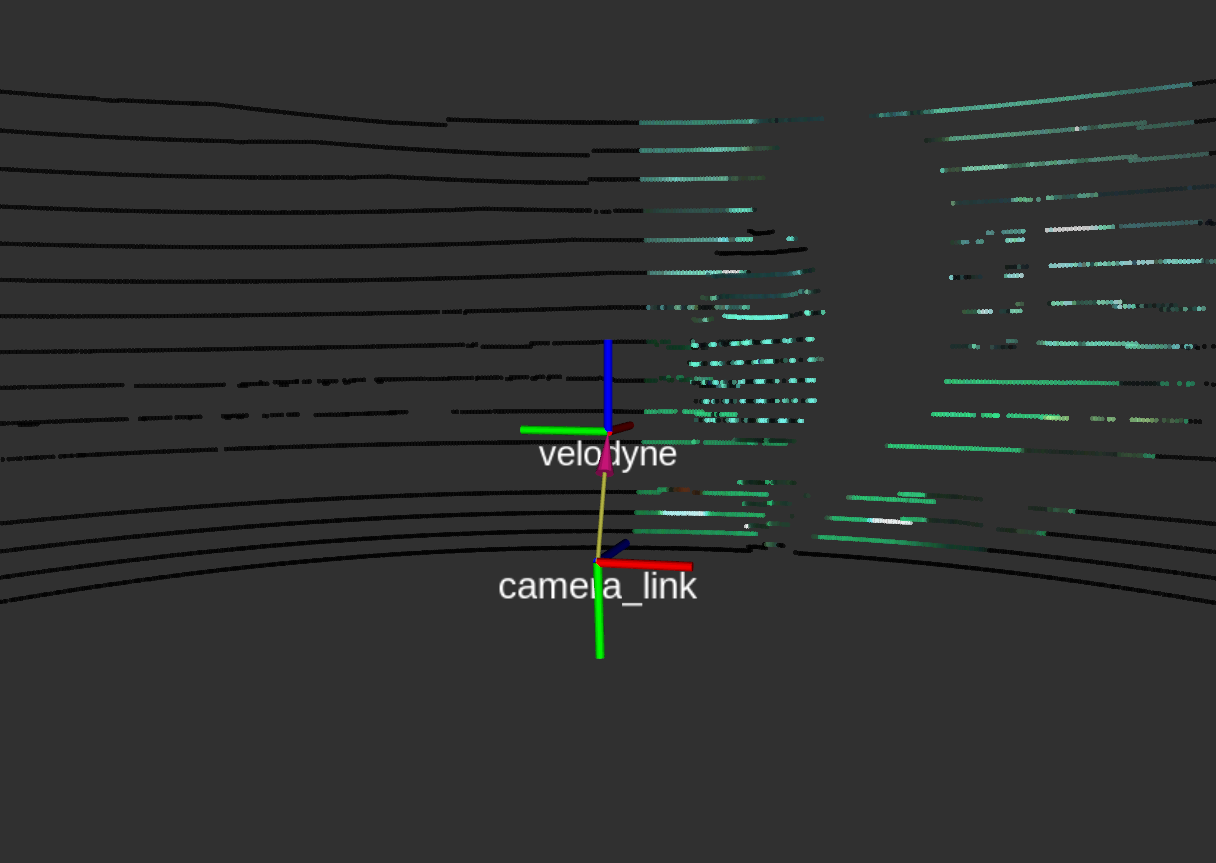
\includegraphics[width=\textwidth]{img/sensor_fusion/cambada_fusion_points.png}
		\caption{}
		\label{fig:sensor-fusion:cambada-points}
	\end{subfigure}
	\qquad
	\begin{subfigure}[t]{0.45\textwidth}
		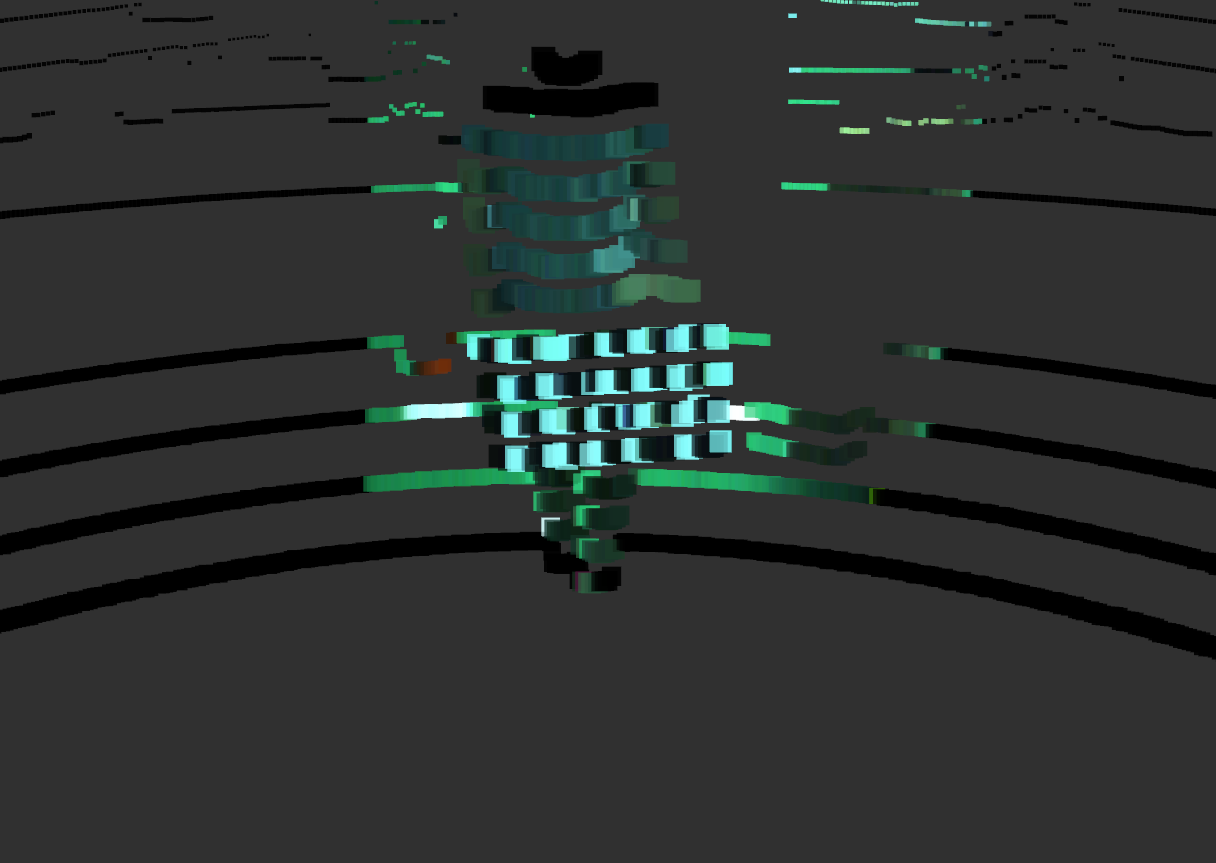
\includegraphics[width=\textwidth]{img/sensor_fusion/cambada_fusion_squares.png}
	\caption{}%The rectangles presented on the image have a size 4 cm and a transparency of 70\%.}
		\label{fig:sensor-fusion:cambada-squares}
	\end{subfigure}
	\caption[Colored point clouds computed for the datasets on \ac{irislab}.]{Data fusion between the camera and the \ac{lidar} on a \ac{msl} field. The colored point cloud is presented on sub-figure: (\subref{fig:sensor-fusion:cambada-points}) with points of 4 pixels and 70\% of transparency, with the coordinate frames also shown; (\subref{fig:sensor-fusion:cambada-squares}) with squares of \SI{4}{\centi\meter} of size and a transparency of 70\%.}
	\label{fig:cambada-sensor-fusion}
\end{figure}

However, such results are obtained with a low point density (VLP-16 only has 16 lines of data\footnote{Actually, our Velodyne VLP-16 has one of its lasers out of order, therefore we only have 15 lines of data.}) and a distance from the objects to the camera (a few meters). 

Another test, from the preliminary stages of the work, show the colored point cloud on \ac{it} 2 Dark Room, a smaller room where some tests were carried. On this case, the objects of interest are closer, so the colored point cloud has a better point cloud density, as shown on Figure~\ref{fig:dark-room-sensor-fusion}, 

\begin{figure}[!ht]
	\centering
	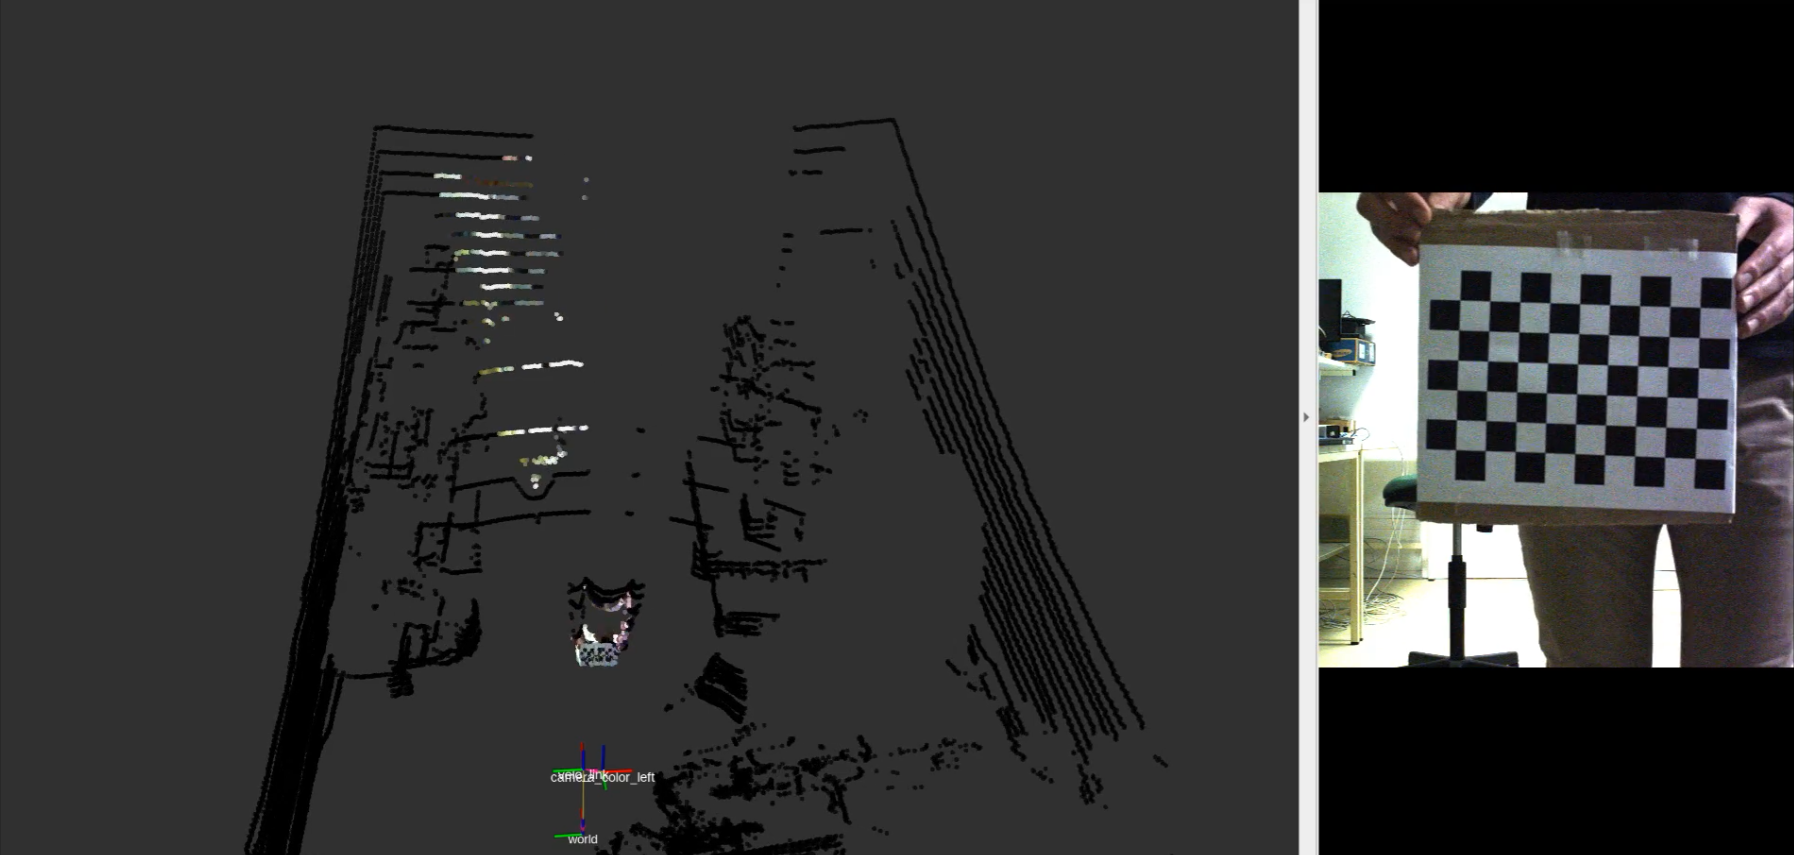
\includegraphics[width=0.7\textwidth]{img/sensor_fusion/dark-room-sensor-fusion.png}
\caption[Example of preliminar data fusion on \ac{it} 2 Dark Room.]{Data fusion between the \ac{lidar} and the camera data. On the left is the colored point cloud and on the right the image. The difference between this and the colored point clouds presented on Figure~\ref{fig:cambada-sensor-fusion} is that the objects of interest are closer to the camera and the experimental setup is placed inside a small room.}
	\label{fig:dark-room-sensor-fusion}
\end{figure}

\subsection{\ac{kitti}}
\label{subsec:sensor-fusion:kitti}
Applying the developed nodes to \ac{kitti} data set, which uses a Velodyne HDL-64E, with 64 pairs of laser beams and photodetectors, having 4 times more lines than our setup, results on the colored point cloud presented in Figure~\ref{fig:kitti-sensor-fusion}. This cloud has some differences when compared with the figures~\ref{fig:cambada-sensor-fusion} and~\ref{fig:dark-room-sensor-fusion}, such as:

\begin{itemize}
	\item The increase of photorealism in the colored point cloud, due to the increase in the number of laser beams;
	\item The dynamic scenario on \ac{kitti} dataset, compared to ours static experimental scenario.
\end{itemize}

On Figure~\ref{fig:kitti-sensor-fusion}, a mismatch between the top and bottom part of the sub-figures can be observed, even if accounting for the different \ac{fov} and view port for the camera and \ac{lidar}. This mismatch is due to the processing delay introduced by the point cloud coloring \ac{ros} node, which results on the colored point cloud being published to the \ac{ros} network with a large delay and our implementation cannot keep up with the publishing demand of \ac{kitti}'s dataset data rate, which causes the mismatch between the points positioning along the car direction of movement. Such mismatch and delay, however, is only due to the hardware  specifications running the algorithm, as is completely eliminated by using a computer with better specifications, specially on \ac{ram}, \ac{gpu} and \ac{cpu}.

\begin{figure}[!ht]
	\centering
	\begin{subfigure}[c]{0.8\textwidth}
		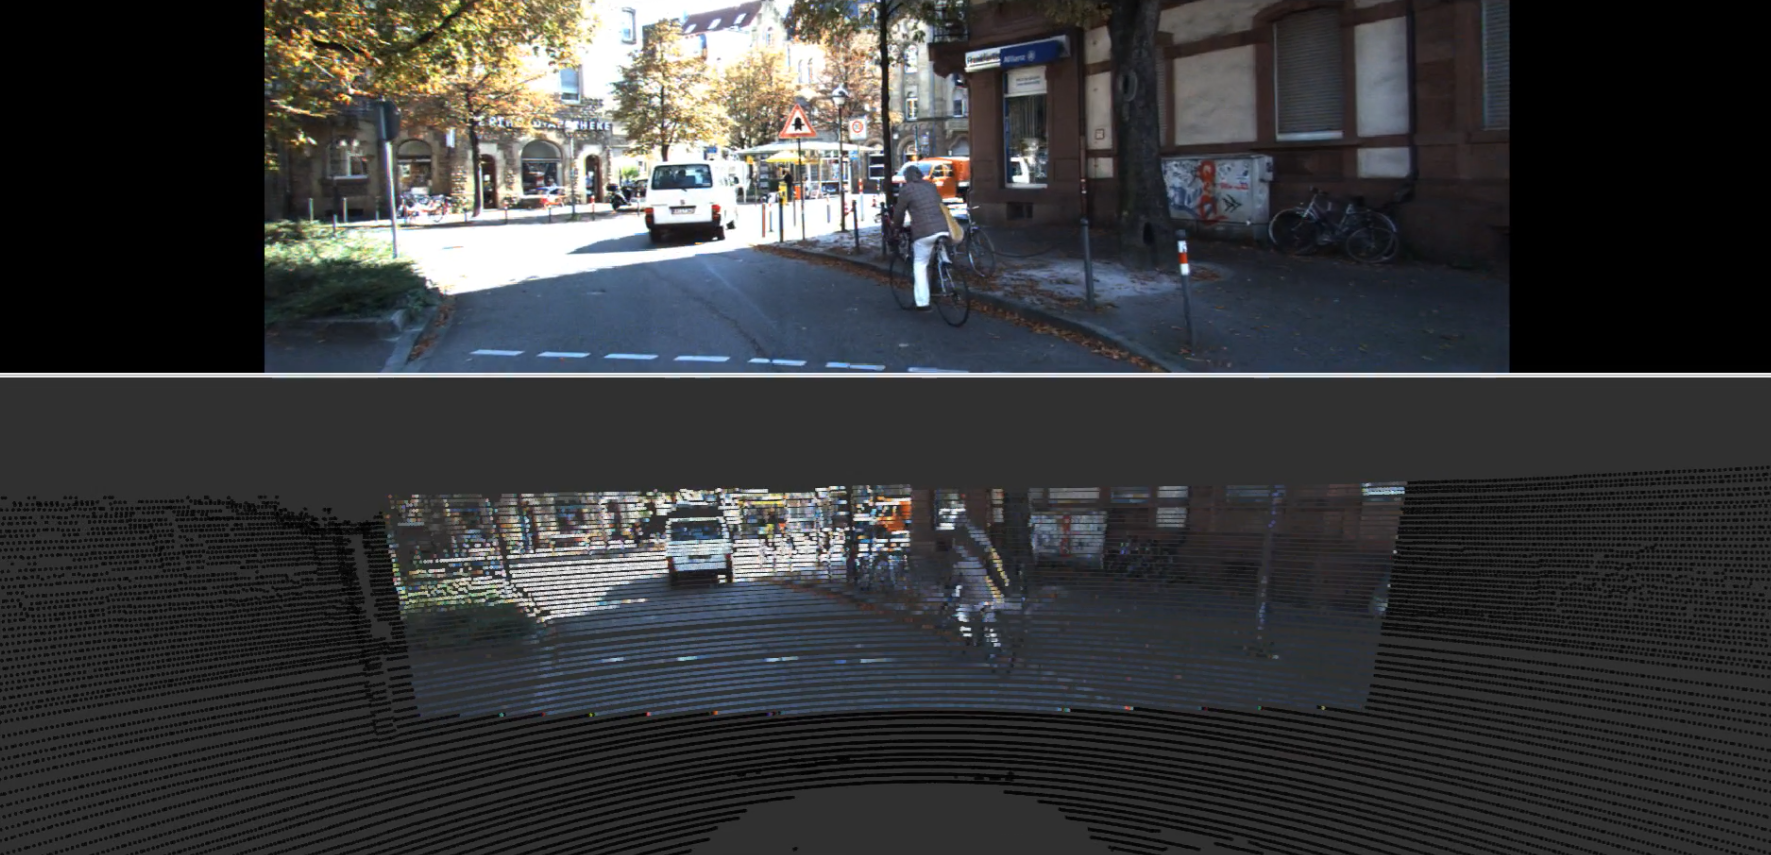
\includegraphics[width=\textwidth]{img/sensor_fusion/kitti-sensor-fusion-1.png}
		\caption{}
		\label{fi		g:kitti-sensor-fusion-1}
	\end{subfigure}
	\\ \vspace{4mm}
	\begin{subfigure}[c]{0.8\textwidth}
		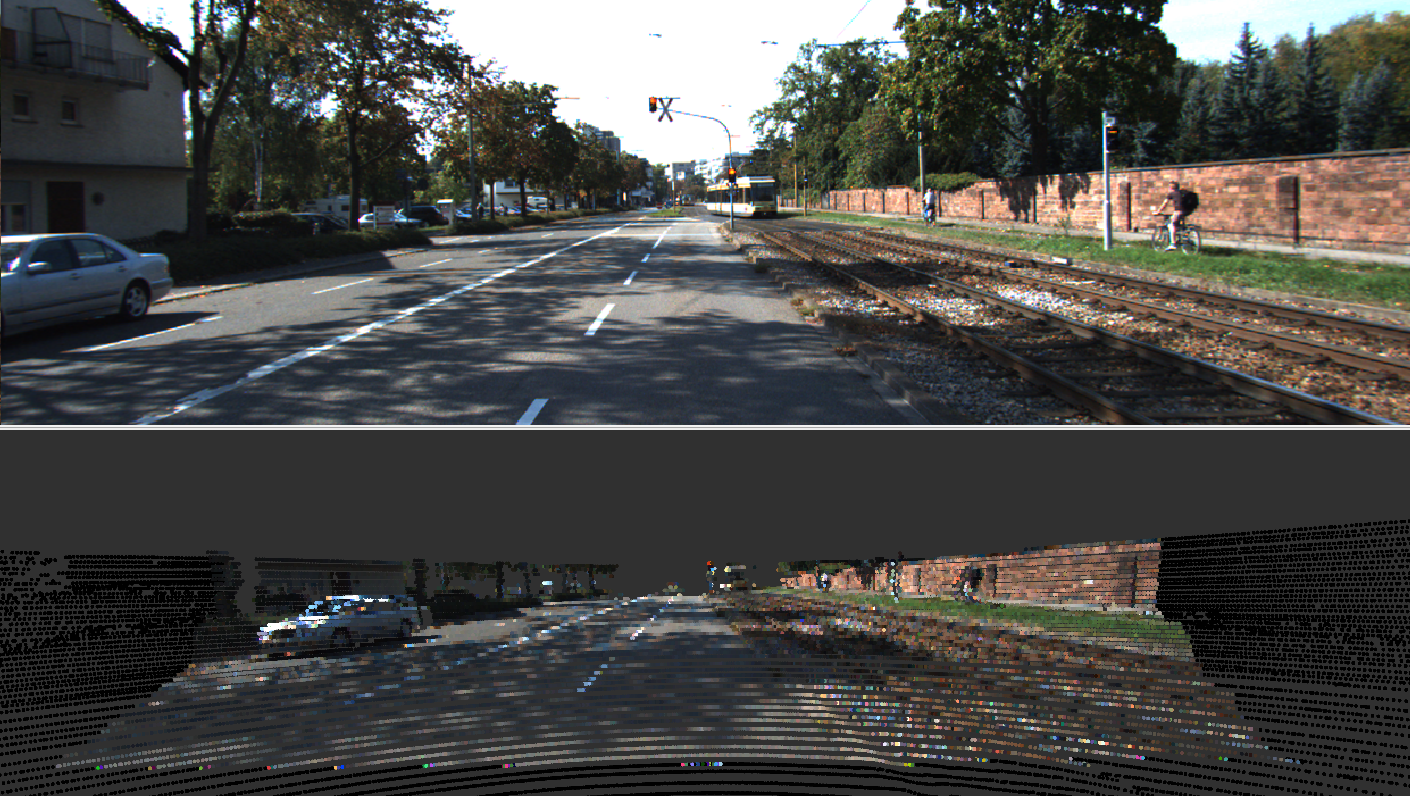
\includegraphics[width=\textwidth]{img/sensor_fusion/kitti-sensor-fusion-2.png}
		\caption{}
		\label{fig:kitti-sensor-fusion-2}
	\end{subfigure}
	\caption{Data fusion between camera and \ac{lidar} applied to the \ac{kitti} dataset. On the top there is the image and on the bottom the colored point cloud, displayed in points with 6 pixels of size and 50\% of transparency. Note that there is a mismatch between the image being shown and the image used to create the colored point cloud of 2 frames. In sub-Figure~(\subref{fig:kitti-sensor-fusion-1}), a cyclist and the car can clearly been identified on the colored point cloud and in sub-Figure~(\subref{fig:kitti-sensor-fusion-2}), the car, the wall, the road lines and the shadows can clearly be seen on the colored point cloud.}
	\label{fig:kitti-sensor-fusion}
\end{figure}


\subsection{Impact of point cloud density}
On Figure~\ref{fig:dark-room-sensor-fusion}, it is evident that coloring a point cloud results on the loss of many high level features that are present on an image. On the resulting colored point cloud can be difficult to distinguish any objects with the original image and if the viewer does not know the scene being displayed.

Such loss of context and high level features is due to the scarce nature of a point cloud in relation to the camera. A 16-beam \ac{lidar} would only have 16 rows of depth data, while a 5\ac{mp} image will have 1920 rows of pixels. That relation means that only 0.83\% of the image rows will have correspondences on the point cloud. Such is the case of our experimental data.

If the number of pixels is considered instead, assuming a high camera \ac{fov} of \SI{90}{\degree} (which is not our case, since monocular camera \ac{fov} is normally lower), a quarter of the point cloud points, $\approx 7200$ points are candidates for correspondences between camera and \ac{lidar}, resulting in only 0.14\% of pixels on the image having a correspondence to the point cloud. 

For \ac{kitti}'s dataset, a 2\ac{mp} camera is used and a 64 beams \ac{lidar}, which yields almost 6\% of the image rows having correspondences and $\approx 5.76\%$ of the image pixels having a corresponding point on the \ac{lidar} point cloud. Comparing with our setup, \ac{kitti} has a number of correspondences between image pixels and point cloud points 41 times higher, which results on the clear difference in photorealism between figures~\ref{fig:cambada-sensor-fusion} and~\ref{fig:dark-room-sensor-fusion} with Figure~\ref{fig:kitti-sensor-fusion}.

Therefore, we can conclude that merging color with the point cloud depth information, on the way we implemented it, is not a feasible solution either to generate better data for autonomous vehicles, assessing the calibration results or possibly mitigating the interference, due to the losses in the information contained on the image. A solution to tackle such scarcity of the \ac{lidar} data and its impacts on point cloud coloring would be to generate a mesh cloud  from a point cloud and then performing mesh cloud coloring and/or interpolation of the point cloud, in order to increase it point cloud density. Obviously, using a \ac{lidar} with a higher number of laser beams will help mitigate this problem.

\section{Final Remarks}
On this chapter, image and point cloud data are fused to create a ``colored point cloud'': a tridimensional point representation of the scene with depth and color information. The perks of such process are detailed on this chapter and a brief discussion of data fusion representation possibilities: color on point cloud points or depth points overlapped on a 2D image. Our implementation chooses the former and two possible implementation are discussed.  

To implement these data fusion, the rigid body transformation between the \ac{lidar} and camera must be determined, following the procedures in Section~\ref{sec:calibration:extrinsic} and the camera and \ac{lidar} must be intrinsically calibrated as indicated in Sections~\ref{sec:calibration:camera} and~\ref{sec:calibration:lidar}. Our implementation, a single online \ac{ros} node, assumes these steps are undertaken and listens to the \ac{lidar} and camera data, synchronizing it and coloring the point cloud. For determine the color of the points, we use the $2D \rightarrow 3D$ correspondences.

The results from this chapter show, visually, that the extrinsic calibration developed on Chapter~\ref{chapter:calibration} is correctly done. However, when comparing the results obtained on \ac{kitti} dataset with ours, our implementation lacks point cloud density to generate a photorealistic colored point cloud. Such drawbacks are caused by the higher \acl{mp} camera and lower number of lasers on our \ac{lidar}, but it reveals that this approach is not the correct one to create better models for autonomous driving. We would have hopped that by using a camera we could help mitigate this problem by merging data together, but this crude approach of projecting data from one coordinate frame to another is not enough. We also discuss briefly the possibility to interpolate the data, to create a better model.


From this chapter, the main outcome is the understanding of transforming and fusing data from one to another, along with some insights on the possibility to use data/sensor fusion to mitigate the \ac{lidar} interference. Also, one takeout are the algorithms and libraries for point cloud to image re-projection, which are used to estimate the point cloud bounding box from the image bounding boxes, on Chapter~\ref{chapter:object-detection} since the mathematical description of the two problems is similar.
